\section{Calculational setup}
\label{sec:setup}
The results presented in this paper have been obtained by combining the two tools
\GoSam~\cite{Cullen:2011ac,Cullen:2014yla} and \Sherpa~\cite{Gleisberg:2008ta}
which allows for a fully automated calculation of cross section and observables and next-to-leading order in QCD as well
as in the electroweak coupling.
\GoSam is a package which generates the code for the numerical evaluation of
the one loop scattering amplitudes starting from the Feynman diagrams,
generated with \QGraf~\cite{Nogueira:1991ex} and further processed with
\FORM~\cite{Vermaseren:2000nd,Kuipers:2012rf} and
\Spinney~\cite{Cullen:2010jv} to perform necessary algebraic
manipulations to obtain an optimized expression for the matrix elements.
For the integrand reduction of the diagrams we use the \Ninja
library~\cite{Peraro:2014cba}, an implementation of the technique of integrand
reduction via Laurent expansion~\cite{Mastrolia:2012bu,vanDeurzen:2013saa}.
Alternatively one can choose other reduction strategies such as OPP reduction
method~\cite{Ossola:2006us,Mastrolia:2008jb,Ossola:2008xq} which is
implemented in $d$ dimensions in \Samurai~\cite{Mastrolia:2010nb}, or methods based on
tensor integral reduction as implemented in
\GolemNF~\cite{Heinrich:2010ax,Binoth:2008uq,Cullen:2011kv,Guillet:2013msa}.
We have used \OneLoop~\cite{vanHameren:2010cp} to evaluate the scalar integrals.

A selection of one-loop amplitudes contributing to the three 
considered processes are shown in Figures 
\ref{fig:aaa:amps}--\ref{fig:aaz:amps}. 
The highest point loop integrals occurring in $\gamma\gamma\gamma$ 
production are pentagons, while both $\gamma\gamma e^-\bar\nu_e$ 
and $\gamma\gamma e^+e^-$ productions include up to hexagons at 
NLO EW. 

\begin{figure}[t!]
  \begin{tabular}{ccccc}
    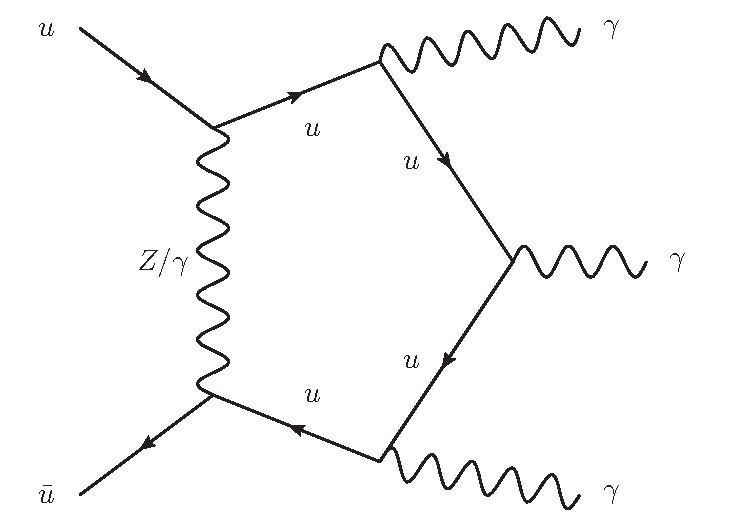
\includegraphics[width=0.288\textwidth]{diagrams/aaa_V_2} & &
    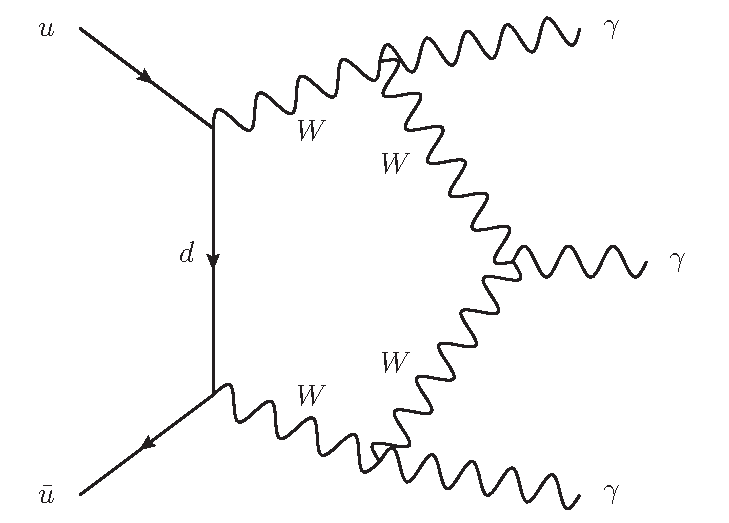
\includegraphics[width=0.288\textwidth]{diagrams/aaa_V_1} & &
    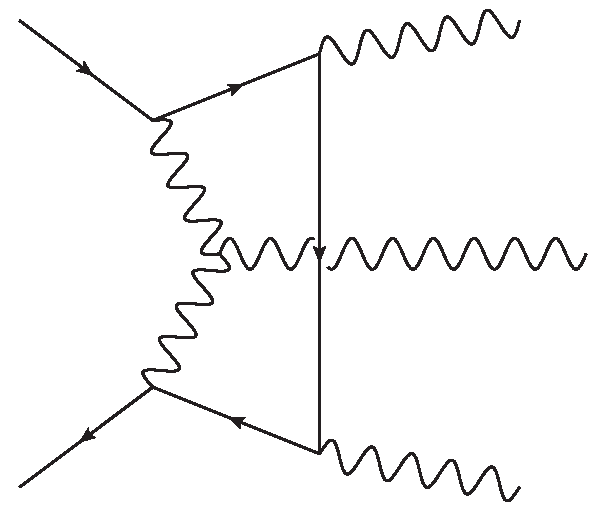
\includegraphics[width=0.288\textwidth]{diagrams/aaa_V_3} \\
  \end{tabular}
  \caption{
    Sample diagrams of electroweak virtual corrections to triple 
    photon production.
    \label{fig:aaa:amps}
  }
\end{figure}

\begin{figure}[t!]
  \begin{tabular}{ccccc}
    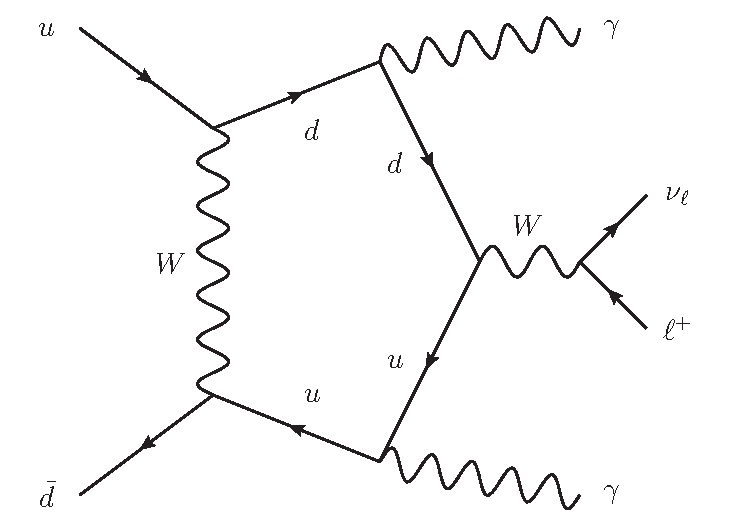
\includegraphics[width=0.288\textwidth]{diagrams/aaW_V_2} & &
    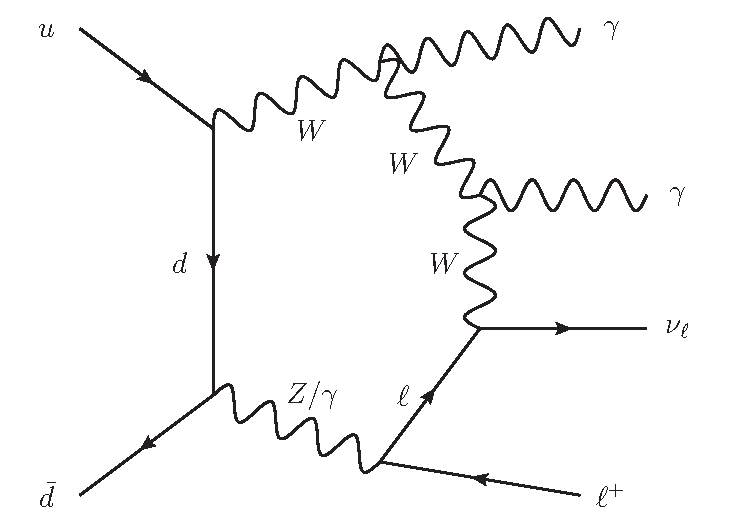
\includegraphics[width=0.288\textwidth]{diagrams/aaW_V_1} & &
    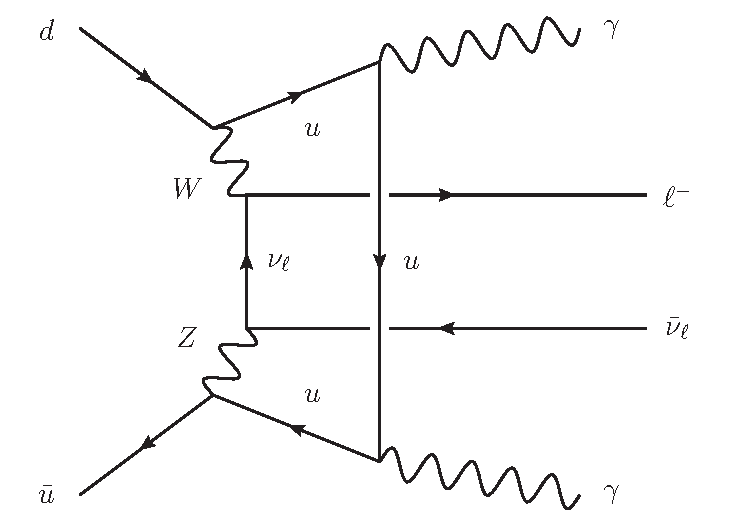
\includegraphics[width=0.288\textwidth]{diagrams/aaW_V_3} \\
  \end{tabular}
  \caption{
    Sample diagrams of electroweak virtual corrections to diphoton 
    production in association with a lepton-neutrino pair.
    \label{fig:aaw:amps}
  }
\end{figure}

\begin{figure}[t!]
  \begin{tabular}{ccccc}
    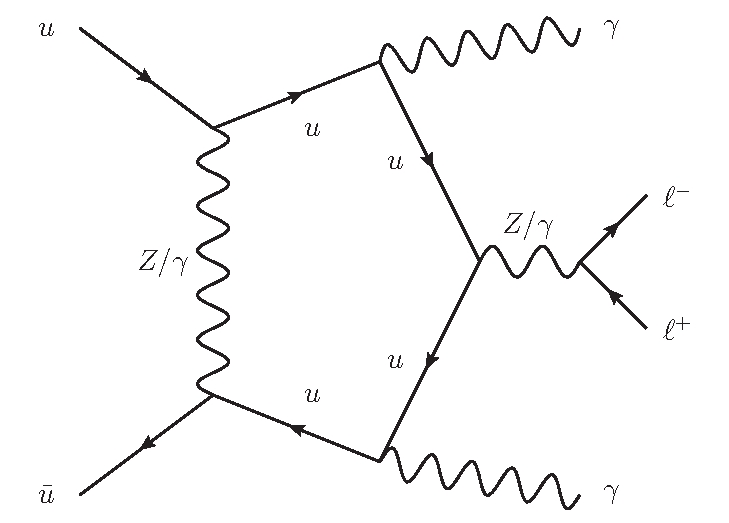
\includegraphics[width=0.288\textwidth]{diagrams/aaZ_V_2} & &
    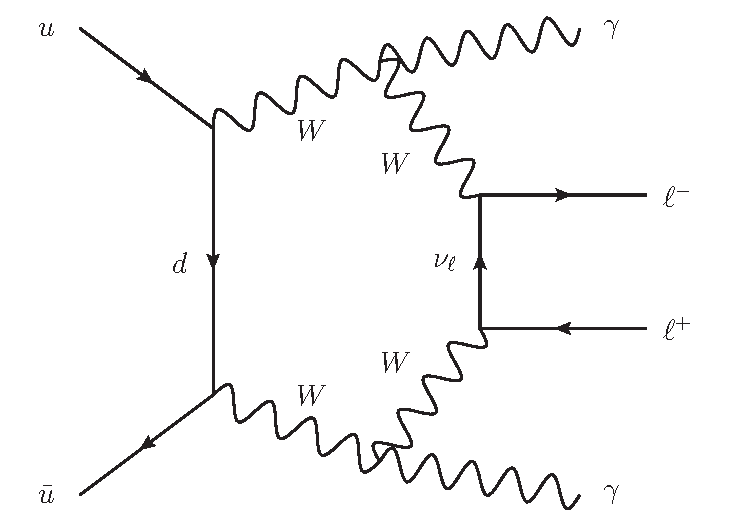
\includegraphics[width=0.288\textwidth]{diagrams/aaZ_V_1} & &
    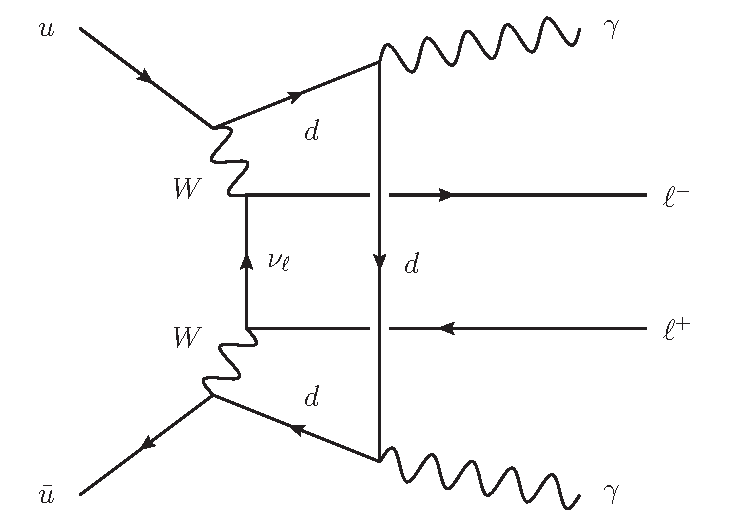
\includegraphics[width=0.288\textwidth]{diagrams/aaZ_V_3} \\
  \end{tabular}
  \caption{
    Sample diagrams of electroweak virtual corrections to diphoton 
    production in association with a lepton-pair.
    \label{fig:aaz:amps}
  }
\end{figure}

\Sherpa, on the other hand, provides the tree-level matrix 
elements, infrared subtraction, process management and phase-space 
integration of all contributions to all processes considered in 
this publication through its tree-level matrix element generator 
\textsc{Amegic} \cite{Krauss:2001iv}. 
Its inbuilt infrared subtraction is performed in the QED 
generalisation of the Catani-Seymour scheme~\cite{Catani:1996vz,
  Dittmaier:1999mb,Gleisberg:2007md,Kallweit:2014xda,
  Kallweit:2015dum,Kallweit:2017khh,Schonherr:2017xxx}
and includes the appropriate initial state mass factorisation 
counter terms.
Both programs, \Sherpa and \GoSam, are interfaced through a 
dedicated interface based on the 
Binoth Les Houches Accord~\cite{Binoth:2010xt,Alioli:2013nda}. 
Cross-checks of the tree-level matrix elements of \GoSam and 
\Sherpa and the renormalized pole coefficients of the virtual 
corrections of \GoSam and the infrared poles of \Sherpa have 
been performed for several phase space points spanning 
multiple kinematic regimes and we have found excellent 
agreement.

This combination of tools was previously used to calculate the 
NLO QCD corrections to $ZZ+\text{jet}$, $t\bar{t}+0,1\,\text{jets}$, 
$W^{+}W^{-}b\bar{b}$ and $h+0,1,2,3\,\text{jets}$ production 
in \cite{Binoth:2009wk,Hoeche:2013mua,Heinrich:2013qaa,
  Greiner:2015jha,Greiner:2016awe,Heinrich:2017bqp} and the 
NLO EW corrections to $\gamma\gamma+0,1,2\,\text{jets}$ production 
in \cite{Chiesa:2017gqx}.
